\documentclass[a4paper]{scrartcl}

\usepackage[
fancytheorems, 
fancyproofs, 
noindent, 
%  spacingfix,  
]{adam}

\usepackage{tikz}
\usetikzlibrary{automata, positioning}

\title{Markov Chains}
\author{Adam Kelly (\texttt{ak2316@cam.ac.uk})}
\date{\today}


\allowdisplaybreaks

\begin{document}

\maketitle

This article constitutes my notes for the `Markov Chains' course, held in Michaelmas 2021 at Cambridge. These notes are \emph{not a transcription of the lectures}, and differ significantly in quite a few areas. Still, all lectured material should be covered.


\tableofcontents

% \clearpage


\section{Introduction}

For this whole course, $I$ will be a finite or countable set. All of our random variables will also be defined on the same probability space $(\Omega, \FF, \PP)$.

\begin{definition}[Markov Chain]
	A \vocab{stochastic process} $(X_n)_{n \geq 0}$ is called a \vocab{Markov chain} if for all $n \geq 0$ and all $x_0, \dots, x_{n+1} \in I$, we have\footnote{We assume here that we are not conditioning on a zero probability event.}
	$$
	\PP(X_{n + 1} = x_{n + 1} \mid X_n = x_n, \dots, X_0 = x_0) = \PP(X_{n + 1} = x_{n + 1} \mid X_n = x_n).
	$$
\end{definition}

\begin{remark}
	This definition gives a \emph{discrete time} Markov chain. It is possible to define a continuous time Markov chain, but we won't worry about that for now.
\end{remark}

If $\PP(X_{n + 1} = y \mid X_n = x)$ for all $x, y \in I$ is independent of $n$, then $X$ is called \vocab{time-homogeneous}. Otherwise, it is \vocab{time-inhomogeneous}. In this course, we will only study time-homogeneous Markov chains.

We will write $P(x, y) = \PP(X_1 = y \mid X_0 = x)$, where $x, y \in I$. We call $P$ a \vocab{stochastic matrix}, because
$$
	\sum_{y \in I} P(x, y) = 1,
$$
that is, the sum of each row is 1.


\begin{remark}
	The index set does not have to be $\N$, it could be say $\{0, 1, \dots, N\}$ for $N \in \N$.
\end{remark}

So to characterize a Markov chain, we need this matrix $P$, giving the probability of passing from a state $x$ to a state $y$. We call this matrix the \vocab{transition matrix} of $X$.

\begin{definition}[Markov]
	We say that $X$ is \vocab{$\markov(\lambda, P)$} if $X_0$ has distribution $\lambda$ and $P$ is the transition matrix. That is,
	\begin{enumerate}[label=(\roman*)]
		\item $\PP(X_0 = x_0) = \lambda_{x_0}$, $x_0 \in I$,
		\item $\PP(X_{n + 1} = x_{n + 1} \mid X_n = x_n, \dots, X_0 = x_0) = P(x_n, x_{n + 1}) = P_{x_n x_{n + 1}}$.
	\end{enumerate}
\end{definition}

We usually represent a Markov chain by its diagram corresponding to the allowed transitions. 

\begin{example}[Diagram of a Markov Chain]
	Let $\alpha, \beta \in (0, 1)$. We consider the matrix
	$$
	P = \begin{pmatrix}
		\alpha & 1 - \alpha \\
		1 - \beta & \beta
	\end{pmatrix}.
	$$
	This is a transition matrix on two states which we can call $1$ and $2$. Here $\alpha$ is the probability of staying at 1, and $1 - \alpha$ is the probability of moving from state 2 when at state 1.

	A diagram of this is given below. This is a directed graph with the relevant probabilities labelling each edge.

	\begin{center}
		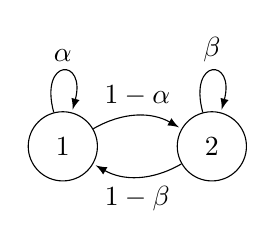
\begin{tikzpicture}

			\node[state] (1) {1};
			\node[state, right=of 1] (2) {2};
			
			\draw[every loop, >=latex]
			(1) edge[loop above] node {$\alpha$} (1)
			(1) edge[bend left, auto=left] node {$1 - \alpha$} (2)
			(2) edge[bend left, auto=left] node {$1 - \beta$} (1)
			(2) edge[loop above] node {$\beta$} (2);
			
			\end{tikzpicture}
	\end{center}
\end{example}

\begin{example}
	Suppose that we have the transition matrix
	$$
	P = \begin{pmatrix}
		\frac{1}{2} & \frac{1}{2} & 0 \\
		\frac{1}{3} & \frac{1}{3} & \frac{1}{3} \\
		1 & 0 & 0 
	\end{pmatrix}.
	$$
	This is a transition matrix on three states and corresponds with the diagram below.

	\begin{center}
		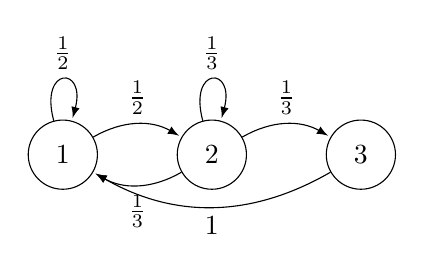
\begin{tikzpicture}
		
		\node[state] (1) {1};
		\node[state, right=of 1] (2) {2};
		\node[state, right=of 2] (3) {3};
		
		\draw[every loop, >=latex]
		(1) edge[loop above] node {$\frac{1}{2}$} (1)
		(1) edge[bend left, auto=left] node {$\frac{1}{2}$} (2)
		(2) edge[bend left, auto=left] node {$\frac{1}{3}$} (1)
		(2) edge[loop above] node {$\frac{1}{3}$} (2)
		(2) edge[bend left, auto=left] node {$\frac{1}{3}$} (3)
		(3) edge[bend left, auto=left] node {$1$} (1);
		
		\end{tikzpicture}
		\end{center}

\end{example}

\begin{theorem}
	The process $X$ is $\markov(\lambda, P)$ if and only if for all $n \geq 0$ and all $x_0, \dots, x_n \in I$ we have
	$$
	\PP(X_0 = x_0, \dots, X_n = x_n) = \lambda_{x_0} P(x_0, x_1) \cdots P(x_{n - 1}, x_n).
	$$
\end{theorem}
\begin{proof}
	First suppose that $X$ is $\markov(\lambda, P)$. Then
	\begin{align*}
		\PP(X_n = x_n, \dots, X_0 = x_0) &= \PP(X_n = x_n \mid X_{n - 1} = x_{n - 1} , \dots, X_0 = x_0) \\&\ \cdot \PP(X_{n - 1} = x_{n - 1} , \dots, X_0 = x_0)\\
		&= P(x_{n - 1}, x_n) \cdot \PP(X_{n - 1} = x_{n - 1} , \dots, X_0 = x_0) \\
		&= P(x_0, x_1) \dots P(x_{n - 1}, x_n) \PP(X_0 = x_0) \\
		&= \lambda_{x_0} P(x_0, x_1) \cdots P(x_{n - 1}, x_n),
	\end{align*}
	as required.

	Now suppose that the property holds. Then $n = 0$ gives $\PP(X_0 = x_0) = \lambda_{x_0}$, so our base case holds. Then
	\begin{align*}
		\PP(X_n = x_)n \mid X_{n - 1} = x_{n - 1} , \dots, X_0 = x_0) &= \frac{\lambda_{x_0}P(x_0, x_1)\cdots P(x_{n - 1}, x_n)}{\lambda_{x_0}P(x_0, x_1)\cdots P(x_{n - 2}, x_{n-1})}\\ 
		&= P(x_{n - 1}, x_n)
	\end{align*}
\end{proof}

Now we are going to define some useful notation.

\begin{definition}[$\delta_i$-mass]
	For $i \in I$, the \vocab{$\delta_i$-mass} of $i$ is defined as
	$\delta_{ij} = \ii(i = j)$.
\end{definition}

Recall the notion of independence for random variables. Let $X_1, \dots, X_n$ be discrete random variables. They are \emph{independent} if for all $x_1, \dots, x_n \in I$, we have
$$
\PP(X_1= x_1, \dots, X_n = x_n) = \prod_{i = 1}^n \PP(X_i = x_i).
$$

We have a similar notion for sequences of random variables. We say a sequence $(X_n)_{n \geq 0}$ is \emph{independent} if for all $i_1 < i_2 < \dots < i_k$ and all $x_1, \dots, x_k$,
$$
\PP(X_{i_1} = x_1, \dots, X_{i_k} = x_k) = \prod_{j = 1}^k \PP(X_{i_j} = x_j).
$$

If $X = (X_n)_{n \geq 0}$ and $Y = (Y_n)_{n \geq 0}$ are two sequences of random variables, they are independent if for all $k, m$ and $i_1 < \cdots < i_k$, $j_1 < \cdots j_m$ we have
\begin{align*}
	&\ \PP(X_{i_1} = x_1, \dots, X_{i_k} = x_k, Y_{j_1} = y_1, \dots, Y_{j_m} = y_m) \\
	&= \PP(X_{i_1} = x_1, \dots, X_{i_k} = x_k) \cdot \PP(Y_{j_1} = y_1, \dots, Y_{j_m} = y_m) 
\end{align*}

\begin{theorem}[Simple Markov Property]
	Suppose that $X$ is $\markov(\lambda, P)$. Fix $m \in \N$ and $i \in I$. Conditional on $X_m = i$, the process $(X_{m + n})_{n \geq 0}$ is $\markov(\delta_i, P)$ and it is independent of $X_0, \dots, X_m$.
\end{theorem}

\begin{proof}
	We need to show that
	$$
	\PP(X_{m} = x_0, \dots, X_{m + n} = x_n \mid X_m = i) = \delta_{i x_0}P(x_0, x_1) \dots P(x_{n - 1}, x_n).
	$$
	(To be completed next lecture)
\end{proof}

\begin{remark}
	Informally, this theorem says `past and future are independent given the present'.
\end{remark}

\end{document}

